% Options for packages loaded elsewhere
\PassOptionsToPackage{unicode}{hyperref}
\PassOptionsToPackage{hyphens}{url}
%
\documentclass[
  14pt,
  letterpaper,
  ignorenonframetext,
  aspectratio=169,
  handout]{beamer}
\usepackage{pgfpages}
\setbeamertemplate{caption}[numbered]
\setbeamertemplate{caption label separator}{: }
\setbeamercolor{caption name}{fg=normal text.fg}
\beamertemplatenavigationsymbolsempty
% Prevent slide breaks in the middle of a paragraph
\widowpenalties 1 10000
\raggedbottom
\setbeamertemplate{part page}{
  \centering
  \begin{beamercolorbox}[sep=16pt,center]{part title}
    \usebeamerfont{part title}\insertpart\par
  \end{beamercolorbox}
}
\setbeamertemplate{section page}{
  \centering
  \begin{beamercolorbox}[sep=12pt,center]{part title}
    \usebeamerfont{section title}\insertsection\par
  \end{beamercolorbox}
}
\setbeamertemplate{subsection page}{
  \centering
  \begin{beamercolorbox}[sep=8pt,center]{part title}
    \usebeamerfont{subsection title}\insertsubsection\par
  \end{beamercolorbox}
}
\AtBeginPart{
  \frame{\partpage}
}
\AtBeginSection{
  \ifbibliography
  \else
    \frame{\sectionpage}
  \fi
}
\AtBeginSubsection{
  \frame{\subsectionpage}
}

\usepackage{amsmath,amssymb}
\usepackage{lmodern}
\usepackage{iftex}
\ifPDFTeX
  \usepackage[T1]{fontenc}
  \usepackage[utf8]{inputenc}
  \usepackage{textcomp} % provide euro and other symbols
\else % if luatex or xetex
  \usepackage{unicode-math}
  \defaultfontfeatures{Scale=MatchLowercase}
  \defaultfontfeatures[\rmfamily]{Ligatures=TeX,Scale=1}
  \setmainfont[Scale=MatchLowercase]{SF Pro Text Light}
  \setmathfont[]{STIX Two Math}
\fi
\usetheme[]{boxes}
\usecolortheme{wolverine}
\usefonttheme{serif} % use mainfont rather than sansfont for slide text
% Use upquote if available, for straight quotes in verbatim environments
\IfFileExists{upquote.sty}{\usepackage{upquote}}{}
\IfFileExists{microtype.sty}{% use microtype if available
  \usepackage[]{microtype}
  \UseMicrotypeSet[protrusion]{basicmath} % disable protrusion for tt fonts
}{}
\makeatletter
\@ifundefined{KOMAClassName}{% if non-KOMA class
  \IfFileExists{parskip.sty}{%
    \usepackage{parskip}
  }{% else
    \setlength{\parindent}{0pt}
    \setlength{\parskip}{6pt plus 2pt minus 1pt}}
}{% if KOMA class
  \KOMAoptions{parskip=half}}
\makeatother
\usepackage{xcolor}
\newif\ifbibliography
\setlength{\emergencystretch}{3em} % prevent overfull lines
\setcounter{secnumdepth}{-\maxdimen} % remove section numbering


\providecommand{\tightlist}{%
  \setlength{\itemsep}{0pt}\setlength{\parskip}{0pt}}\usepackage{longtable,booktabs,array}
\usepackage{calc} % for calculating minipage widths
\usepackage{caption}
% Make caption package work with longtable
\makeatletter
\def\fnum@table{\tablename~\thetable}
\makeatother
\usepackage{graphicx}
\makeatletter
\def\maxwidth{\ifdim\Gin@nat@width>\linewidth\linewidth\else\Gin@nat@width\fi}
\def\maxheight{\ifdim\Gin@nat@height>\textheight\textheight\else\Gin@nat@height\fi}
\makeatother
% Scale images if necessary, so that they will not overflow the page
% margins by default, and it is still possible to overwrite the defaults
% using explicit options in \includegraphics[width, height, ...]{}
\setkeys{Gin}{width=\maxwidth,height=\maxheight,keepaspectratio}
% Set default figure placement to htbp
\makeatletter
\def\fps@figure{htbp}
\makeatother

\captionsetup[figure]{labelformat=empty}
\usepackage{pgfpages}
\setbeamertemplate{itemize item}[circle]
\setbeamertemplate{footline}[frame number]{}
\mode<handout>{\pgfpagesuselayout{6 on 1}[letterpaper, border shrink=8mm]}
\AtBeginSection{%
   \begin{frame}
       \tableofcontents[currentsection]
   \end{frame}
   }
\usepackage{tikz}
\usetikzlibrary{positioning,arrows,calc}
\usepackage{tikz-qtree}
\tikzset{
   modal/.style={>=stealth',
   shorten >=1pt,
   shorten <=1pt,
   auto,
   node distance=1.5cm,
   label distance=2pt,
   semithick},
 every label/.style={phantom,align=left},
 world/.style = {circle,draw,minimum size=0.5cm,fill=gray!15},
 modal every node/.style={world},
 point/.style={circle,draw,inner sep=0.5mm,fill=black},
 phantom/.style={rectangle,inner sep=0pt,draw=none,fill=none},
 reflexive above/.style={->,loop,looseness=7,in=60,out=120},
 reflexive below/.style={->,loop,looseness=7,in=240,out=300},
 reflexive left/.style={->,loop,looseness=7,in=150,out=210},
 reflexive right/.style={->,loop,looseness=7,in=30,out=330}
 }
\makeatletter
\makeatother
\makeatletter
\makeatother
\makeatletter
\@ifpackageloaded{caption}{}{\usepackage{caption}}
\AtBeginDocument{%
\ifdefined\contentsname
  \renewcommand*\contentsname{Table of contents}
\else
  \newcommand\contentsname{Table of contents}
\fi
\ifdefined\listfigurename
  \renewcommand*\listfigurename{List of Figures}
\else
  \newcommand\listfigurename{List of Figures}
\fi
\ifdefined\listtablename
  \renewcommand*\listtablename{List of Tables}
\else
  \newcommand\listtablename{List of Tables}
\fi
\ifdefined\figurename
  \renewcommand*\figurename{Figure}
\else
  \newcommand\figurename{Figure}
\fi
\ifdefined\tablename
  \renewcommand*\tablename{Table}
\else
  \newcommand\tablename{Table}
\fi
}
\@ifpackageloaded{float}{}{\usepackage{float}}
\floatstyle{ruled}
\@ifundefined{c@chapter}{\newfloat{codelisting}{h}{lop}}{\newfloat{codelisting}{h}{lop}[chapter]}
\floatname{codelisting}{Listing}
\newcommand*\listoflistings{\listof{codelisting}{List of Listings}}
\makeatother
\makeatletter
\@ifpackageloaded{caption}{}{\usepackage{caption}}
\@ifpackageloaded{subcaption}{}{\usepackage{subcaption}}
\makeatother
\makeatletter
\@ifpackageloaded{tcolorbox}{}{\usepackage[many]{tcolorbox}}
\makeatother
\makeatletter
\@ifundefined{shadecolor}{\definecolor{shadecolor}{rgb}{.97, .97, .97}}
\makeatother
\makeatletter
\makeatother
\ifLuaTeX
  \usepackage{selnolig}  % disable illegal ligatures
\fi
\IfFileExists{bookmark.sty}{\usepackage{bookmark}}{\usepackage{hyperref}}
\IfFileExists{xurl.sty}{\usepackage{xurl}}{} % add URL line breaks if available
\urlstyle{same} % disable monospaced font for URLs
\hypersetup{
  pdftitle={Honors Logic, Lecture 10 - Modal Logic},
  pdfauthor={Brian Weatherson},
  hidelinks,
  pdfcreator={LaTeX via pandoc}}

\title{Honors Logic, Lecture 10 - Modal Logic}
\author{Brian Weatherson}
\date{2022-09-30}

\begin{document}
\frame{\titlepage}
\ifdefined\Shaded\renewenvironment{Shaded}{\begin{tcolorbox}[sharp corners, enhanced, boxrule=0pt, interior hidden, breakable, borderline west={3pt}{0pt}{shadecolor}, frame hidden]}{\end{tcolorbox}}\fi

\begin{frame}{What Modal Logic Is}
\protect\hypertarget{what-modal-logic-is}{}
The logics of \textbf{must} and \textbf{might}.

\begin{itemize}[<+->]
\tightlist
\item
  Why plural? Because we do not assume that these words have a single
  determinate meaning.
\end{itemize}
\end{frame}

\begin{frame}{Examples of Must}
\protect\hypertarget{examples-of-must}{}
\begin{enumerate}[<+->]
\tightlist
\item
  If \(x = 2 + 2\), then \(x\) must equal 4.
\item
  If something is a cat, then it must be a mammal.
\item
  If the gardener is innocent, then it must be the butler who did it.
\item
  You must drive under 70mph on I-94.
\item
  You must keep your promises.
\item
  If you set out a knife and fork, the fork must go on the left.
\end{enumerate}

\begin{itemize}[<+->]
\tightlist
\item
  To my ears, 1 is \textbf{logical} necessity, 2 is
  \textbf{metaphysical} necessity, 3 is \textbf{epistemic} necessity, 4
  is \textbf{legal} necessity, 5 is \textbf{moral} (or \textbf{deontic})
  necessity and 6 is \textbf{etiquette} necessity.
\end{itemize}
\end{frame}

\begin{frame}{Examples of May/Might}
\protect\hypertarget{examples-of-maymight}{}
\begin{enumerate}[<+->]
\tightlist
\item
  If \(x\) is prime, then \(x\) might be even.
\item
  If \(x\) is a cat, then \(x\) might be male.
\item
  It might be the butler or the gardener that did it.
\item
  You may drive at any speed below 30mph on State Street.
\item
  You may lie to save a friend's life.
\item
  You may use white napkins or red napkins.
\end{enumerate}

\begin{itemize}[<+->]
\tightlist
\item
  To my ears, 1 is \textbf{logical} possibility, 2 is
  \textbf{metaphysical} possibility, 3 is \textbf{epistemic}
  possibility, 4 is \textbf{legal} possibility, 5 is \textbf{moral} (or
  \textbf{deontic}) possibility and 6 is \textbf{etiquette} possibility
  (though I'm not sure about any of these).
\end{itemize}
\end{frame}

\begin{frame}{Logics}
\protect\hypertarget{logics}{}
Consider this very general claim.

\begin{quote}
If something must be true, then it is true.
\end{quote}

\begin{itemize}[<+->]
\tightlist
\item
  That's true on the logical, epistemic and metaphysical interpretations
  of modality. \pause Indeed, it's something like a logical truth of
  those domains.
\item
  But it is very much not true on the legal, moral or etiquette
  interpretations.
\end{itemize}

So we want some logics where it is a logical truth, and some where it is
not.
\end{frame}

\begin{frame}{Language}
\protect\hypertarget{language}{}
We extend our language with two new operators: \(\Box\) and
\(\Diamond\).

\begin{itemize}[<+->]
\tightlist
\item
  If \(p\) is a sentence, so is \(\Box p\) and so is \(\Diamond p\).
\item
  These mean, respectively, that \(p\) must be true, and that \(p\)
  might be true.
\item
  We interpret these somewhat similar to negations; they just bind what
  they are immediately next to.
\item
  So \(\Box p \rightarrow q\) means \((\Box p) \rightarrow q\), not
  \(\Box(p \rightarrow q)\).
\end{itemize}
\end{frame}

\begin{frame}{Truth}
\protect\hypertarget{truth}{}
What does it take for these sentences to be true?
\end{frame}

\begin{frame}{Worlds}
\protect\hypertarget{worlds}{}
We start with Leibniz's idea that necessity is truth in all possible
worlds.

\begin{itemize}[<+->]
\tightlist
\item
  Leibniz was interested in metaphysical necessity, so we'll have to
  qualify this a little, but it's a good idea.
\item
  So instead of saying that each proposition simply has a truth value,
  we'll say that there are many \textbf{worlds}, and at each world each
  proposition has a truth value.
\item
  But don't assume that propositions have the same truth value at each
  world.
\item
  In one world I might be standing, and in another world I might be
  sitting.
\end{itemize}
\end{frame}

\begin{frame}{What Are Worlds}
\protect\hypertarget{what-are-worlds}{}
We are well and truly not going to get into the metaphysics of worlds
here.

\begin{itemize}[<+->]
\tightlist
\item
  Indeed, they need not even be anything like possible worlds in the
  sense that metaphysicians usually care about.
\item
  They might, for instance, be different times.
\item
  All we care about is that they are things at which propositions can be
  true or false.
\end{itemize}
\end{frame}

\begin{frame}{Valuations}
\protect\hypertarget{valuations}{}
A valuation function tells us which worlds atomic sentences are true at.

\begin{itemize}[<+->]
\tightlist
\item
  These can be completely arbitrary; we don't put any restrictions on
  them.
\end{itemize}
\end{frame}

\begin{frame}{Truth at a World}
\protect\hypertarget{truth-at-a-world}{}
We want more generally a function that tells us whether a sentence is
true at a particular world.

\begin{itemize}[<+->]
\tightlist
\item
  For sentences built up using \(\wedge, \vee, \rightarrow, \neg\), this
  is relatively easy.
\item
  We just keep on using truth tables.
\item
  So if at world \(w\), \(A\) is true and \(B\) is false, then
  \(A \wedge B\) is false and \(A \vee B\) is true.
\end{itemize}
\end{frame}

\begin{frame}{Modal Values}
\protect\hypertarget{modal-values}{}
We also need values for these sentences:

\begin{itemize}[<+->]
\tightlist
\item
  \(\Box A\)
\item
  \(\Diamond A\)
\end{itemize}

It turns out these are more complicated - but not much more complicated.
\end{frame}

\begin{frame}{Accessibility}
\protect\hypertarget{accessibility}{}
The last part of our model is an \textbf{accessibility} relation between
worlds.

\begin{itemize}[<+->]
\tightlist
\item
  Again, this can be completely arbitrary.
\item
  We don't yet put any restrictions on it.
\item
  Notably, we don't assume that it is \textbf{reflexive},
  \textbf{symmetric} or \textbf{transitive}
\end{itemize}
\end{frame}

\begin{frame}{Properties of Relations}
\protect\hypertarget{properties-of-relations}{}
\begin{itemize}[<+->]
\tightlist
\item
  \(R\) is reflexive iff for all \(x\), \(xRx\).
\item
  \(R\) is symmetric iff for all \(x, y\), if \(xRy\) then \(yRx\).
\item
  \(R\) is transitive iff for all \(x, y, z\) if \(xRy\) and \(yRz\)
  then \(xRz\).
\end{itemize}

A lot of relations we care about have one or more of these properties,
but not all do. Consider, for example, \textbf{admires} as an example of
a relation with none of them.
\end{frame}

\begin{frame}{Truth of Modal Formulas}
\protect\hypertarget{truth-of-modal-formulas}{}
A sentence \(\Box A\) is true at a world \(x\) just in case the
following condition is met:

\begin{itemize}[<+->]
\tightlist
\item
  For all worlds \(y\) such that \(xRy\), \(A\) is true at world \(y\).
\end{itemize}

A sentence \(\Diamond A\) is true at a world \(x\) just in case the
following condition is met:

\begin{itemize}[<+->]
\tightlist
\item
  For some world \(y\) such that \(xRy\), \(A\) is true at world \(y\).
\end{itemize}
\end{frame}

\begin{frame}{Modal Truth}
\protect\hypertarget{modal-truth}{}
\begin{itemize}[<+->]
\tightlist
\item
  Something is necessarily true iff it is true everywhere that is
  accessible.
\item
  Something is possibly true iff it is true somewhere accessible.
\end{itemize}

We get back the Leibnizian idea that necessity is truth in all possible
worlds if we assume the accessibility relation is the universal
relation, i.e., \(xRy\) for all \(x, y\).
\end{frame}

\begin{frame}{Metaphysical Necessity}
\protect\hypertarget{metaphysical-necessity}{}
On this Leibnizian model, where all worlds can access all worlds,
iterated modalities are rather uninteresting. These three sentences are
true in the same worlds/models.

\begin{enumerate}[<+->]
\tightlist
\item
  \(\Box A\)
\item
  \(\Box \Box A\)
\item
  \(\Diamond \Box A\)
\end{enumerate}

\begin{itemize}[<+->]
\tightlist
\item
  That's because if \(\Box A\) is true at any world, then it is true at
  all worlds. In the general case, where we do not assume that \(R\) is
  universal, these are not equivalent.
\end{itemize}
\end{frame}

\begin{frame}{Duality}
\protect\hypertarget{duality}{}
These two claims are equivalent.

\begin{enumerate}[<+->]
\tightlist
\item
  \(\Box A\)
\item
  \(\neg \Diamond \neg A\)
\end{enumerate}

From 1 to 2: If \(\Box A\) is true at \(x\), then \(A\) is true for all
\(y\) such that \(xRy\). That means there is no \(y\) such that \(xRy\)
and \(A\) is not true. That means there is no \(y\) such that \(xRy\)
and \(\neg A\) is true. That means \(\Diamond \neg A\) is not true at
\(w\). That means \(\neg \Diamond \neg A\) is true at \(x\).
\end{frame}

\begin{frame}{Duality}
\protect\hypertarget{duality-1}{}
These two claims are equivalent.

\begin{enumerate}[<+->]
\tightlist
\item
  \(\Box A\)
\item
  \(\neg \Diamond \neg A\)
\end{enumerate}

From 2 to 1: If \(\neg \Diamond \neg A\) is true at \(x\), then
\(\Diamond \neg A\) is not true at \(w\). So there is no world \(y\)
such that \(xRy\) and \(\neg A\) is true at \(y\). So at all worlds
\(y\) such that \(xRy\), \(\neg A\) is not true. So at all worlds \(y\)
such that \(xRy\), \(A\) is true. So \(\Box A\) is true at \(x\).
\end{frame}

\begin{frame}{Duality}
\protect\hypertarget{duality-2}{}
These two claims are also equivalent, though I will not prove this.

\begin{enumerate}[<+->]
\tightlist
\item
  \(\Diamond A\)
\item
  \(\neg \Box \neg A\)
\end{enumerate}
\end{frame}

\begin{frame}{Big Picture}
\protect\hypertarget{big-picture}{}
These claims are both logically true.

\begin{enumerate}[<+->]
\tightlist
\item
  \(\Box \neg A \leftrightarrow \neg \Diamond A\)
\item
  \(\Diamond \neg A \leftrightarrow \neg \Box A\)
\end{enumerate}

To move a negation sign outside of a modal operator, either \(\Box\) or
\(\Diamond\), you have to rotate the operator by 45 degrees.
\end{frame}

\begin{frame}{Normality}
\protect\hypertarget{normality}{}
This sentence is also true no matter what the model looks like, and no
matter what sentence \(A\) is.

\begin{quote}
\(\Box (A \rightarrow B) \rightarrow (\Box A \rightarrow \Box B)\)
\end{quote}

\begin{itemize}[<+->]
\tightlist
\item
  Assume it is false at \(w\).
\item
  So \(\Box (A \rightarrow B)\) is true at \(w\) and
  \((\Box A \rightarrow \Box B)\) is false at \(w\).
\item
  So \(\Box A\) is true at \(w\) and \(\Box B\) is false at \(w\).
\item
  So at every where \(y\) such that \(wRy\), \(A\) must be true (since
  \(\Box A\) is true at \(w\)), and \(A \rightarrow B\) must be true
  (since \(\Box(A \rightarrow B)\) is true at \(w\)).
\item
  If \(A\) and \(A \rightarrow B\) are true at \(y\), \(B\) must be true
  at \(y\) as well.
\item
  But this implies that \(B\) is true all \(y\) such that \(wRy\),
  contradicting the assumption that \(\Box B\) is false at \(w\).
\end{itemize}
\end{frame}

\begin{frame}{Normality}
\protect\hypertarget{normality-1}{}
This principle has a very important role in the history of modal logics.

\begin{quote}
\(\Box (A \rightarrow B) \rightarrow (\Box A \rightarrow \Box B)\)
\end{quote}

Having this be an axiom is one of two conditions on what have come to be
called \textbf{normal} modal logics.
\end{frame}

\begin{frame}{Models}
\protect\hypertarget{models}{}
Models have three parts:

\begin{enumerate}[<+->]
\tightlist
\item
  A set of worlds, typically called \(W\).
\item
  A binary accessibility relation on those worlds, typically called
  \(R\).
\item
  A valuation function on those worlds, typically called \(V\).
\end{enumerate}

We'll write the models as \(\langle W, R, V\rangle\).
\end{frame}

\begin{frame}{Valuations}
\protect\hypertarget{valuations-1}{}
\(V\) is a function from atomic sentence letters to subsets of \(W\).

\begin{itemize}[<+->]
\tightlist
\item
  It tells you when the atomic sentences are true.
\item
  When an atomic sentence is not true, it is false.
\end{itemize}
\end{frame}

\begin{frame}{Truth at a Point}
\protect\hypertarget{truth-at-a-point}{}
The general theory of truth is built up in stages from the basic theory.
Assume we have a model \(\langle W, R, V\rangle\), and a point
\(w \in W\), and are asking whether an arbitrary sentence is true at
\(w\) in \(\langle W, R, V\rangle\).

\begin{itemize}[<+->]
\tightlist
\item
  \(p\) is true at \(w\) iff \(w \in V(p)\).
\item
  \(\neg A\) is true at \(w\) iff \(A\) is not true at \(w\).
\item
  \(A \wedge B\) is true at \(w\) iff \(A\) is true and \(w\) and \(B\)
  is true at \(w\).
\item
  \(A \vee B\) is true at \(w\) iff \(A\) is true and \(w\) or \(B\) is
  true at \(w\).
\item
  \(A \rightarrow B\) is true at \(w\) iff \(A\) is false at \(w\) or
  \(B\) is true at \(w\).
\end{itemize}

This just leaves the modal formulae. I'll set out the rules, then do
some worked examples.
\end{frame}

\begin{frame}{Necessary Truth at a Point}
\protect\hypertarget{necessary-truth-at-a-point}{}
First we'll do \(\Box A\).

\begin{itemize}[<+->]
\tightlist
\item
  I'll read this as `Box \(A\)'.
\item
  Intuitively, it means \textbf{It must be that A}, where \textbf{must}
  could be a metaphysical necessity, or an epistemic necessity, or a
  moral necessity, or anything else.
\item
  And it is true at \(w\) just in case \(A\) is true at every world
  \(y\) such that \(wRy\).
\item
  Necessary truth is truth at all accessible worlds.
\end{itemize}
\end{frame}

\begin{frame}{Possible Truth at a Point}
\protect\hypertarget{possible-truth-at-a-point}{}
Now we'll do \(\Diamond A\).

\begin{itemize}[<+->]
\tightlist
\item
  I'll read this as `Diamond \(A\)'.
\item
  Intuitively, it means \textbf{It might be that A}, where
  \textbf{might} could be a metaphysical necessity, or an epistemic
  necessity, or a moral necessity, or anything else.
\item
  And it is true at \(w\) just in case \(A\) is true at some world \(y\)
  such that \(wRy\).
\item
  Possible truth is truth at some accessible world.
\end{itemize}
\end{frame}

\begin{frame}{Iterated Modalities}
\protect\hypertarget{iterated-modalities}{}
We can run these rules in sequence.

\begin{itemize}[<+->]
\tightlist
\item
  What does it take for \(\Box \Box A\) to be true at \(w\)?
\item
  It is for \(\Box A\) to be true at every \(y\) such that \(wRy\).
\item
  And that means that \(A\) has to be true at every world \(z\) such
  that \(yRz\) (for any \(y\) such that \(wRy)\).
\end{itemize}
\end{frame}

\begin{frame}{Access}
\protect\hypertarget{access}{}
We can think, a little picturesquely, as the accessibility relation
being a `step' between worlds.

\begin{itemize}[<+->]
\tightlist
\item
  If \(wRy\), then you can `step' from \(w\) to \(y\).
\item
  \(\Box A\) means that anywhere you can step to from \(w\) is a world
  where \(A\) is true.
\item
  And \(\Box \Box A\) means that anywhere you can get to in two steps
  from \(w\) is a world where \(A\) is true.
\end{itemize}
\end{frame}

\begin{frame}{Iterated Modalities}
\protect\hypertarget{iterated-modalities-1}{}
We can run the rules in sequence.

\begin{itemize}[<+->]
\tightlist
\item
  What does it take for \(\Diamond \Diamond A\) to be true at \(w\)?
\item
  It is for \(\Diamond A\) to be true at some \(y\) such that \(wRy\).
\item
  And that means that \(A\) has to be true at some world \(z\) such that
  \(yRz\) (for some \(y\) such that \(wRy)\).
\item
  In the picturesque terms, you can get from \(w\) to an \(A\)-world in
  two steps.
\end{itemize}
\end{frame}

\begin{frame}{Mixed Modalities}
\protect\hypertarget{mixed-modalities}{}
What does it mean for \(\Diamond \Box A\) to be true at \(w\)?

\begin{itemize}[<+->]
\tightlist
\item
  There is some accessible world where \(\Box A\) is true.
\item
  That is, there is some accessible world such that everywhere you can
  go from there, \(A\) is true.
\end{itemize}
\end{frame}

\begin{frame}{Mixed Modalities}
\protect\hypertarget{mixed-modalities-1}{}
What does it mean for \(\Box \Diamond A\) to be true at \(w\)?

\begin{itemize}[<+->]
\tightlist
\item
  At all accessible worlds, \(\Diamond A\) is true.
\item
  That is, wherever you go, you can get to there is some accessible
  world such that everywhere you can go from there, \(A\) is true.
\end{itemize}
\end{frame}

\begin{frame}{Longer Sentences}
\protect\hypertarget{longer-sentences}{}
What does it mean for \(\Box(p \vee (q \rightarrow \Diamond r))\) to be
true at \(w\)?

\begin{itemize}[<+->]
\tightlist
\item
  It's for \(p \vee (q \rightarrow \Diamond r)\) to be true everywhere
  you can get to (in one step) from \(w\).
\item
  That is, at every one of those worlds, either \(p\) is true or
  \(q \rightarrow \Diamond r\) is true.
\item
  That is, at every one of those worlds, either \(p\) is true, or \(q\)
  is false, or \(\Diamond r\) is true.
\item
  That is, at every one of those worlds, either \(p\) is true, or \(q\)
  is false, or there is some world you can get to where \(r\) is true.
\end{itemize}
\end{frame}

\begin{frame}{Box and connectives}
\protect\hypertarget{box-and-connectives}{}
The general rule is just to apply the rules for sentences inside the
brackets at each world in \(W\), and then apply the rule for \(\Box\) or
\(\Diamond\). But there are three special cases worth thinking about.

\begin{itemize}[<+->]
\tightlist
\item
  \(\Box(A \wedge B)\) means that all accessible worlds are \(A\) and
  \(B\) worlds.
\item
  \(\Box(A \vee B)\) means that all accessible worlds make at least one
  of \(A\) and \(B\) true.
\item
  \(\Box(A \rightarrow B)\) means that all accessible \(A\)-worlds are
  \(B\)-worlds.
\end{itemize}

We'll use that last one a lot.
\end{frame}

\begin{frame}
I'm going to go through some sentences, and show how there can be models
where each of them is false. Here is what we'll cover

\begin{enumerate}[<+->]
\tightlist
\item
  \(\Box(A \vee B) \rightarrow (\Box A \vee \Box B)\)
\item
  \((\Diamond A \wedge \Diamond B) \rightarrow \Diamond (A \wedge B)\)
\item
  \(A \rightarrow \Box A\)
\item
  \(\Box A \rightarrow A\)
\item
  \(\Box \Diamond A \rightarrow B\)
\item
  \(\Box \Diamond A \rightarrow A\)
\item
  \(\Box \Box A \rightarrow \Box A\)
\item
  \(\Box A \rightarrow \Box \Box A\)
\item
  \(\Box \Diamond A \rightarrow \Diamond \Box A\)
\item
  \(\Box A \rightarrow \Diamond A\)
\end{enumerate}
\end{frame}

\begin{frame}{\(\Box(A \vee B) \rightarrow (\Box A \vee \Box B)\)}
\protect\hypertarget{boxa-vee-b-rightarrow-box-a-vee-box-b}{}
\begin{columns}
    \begin{column}{0.65\textwidth}
        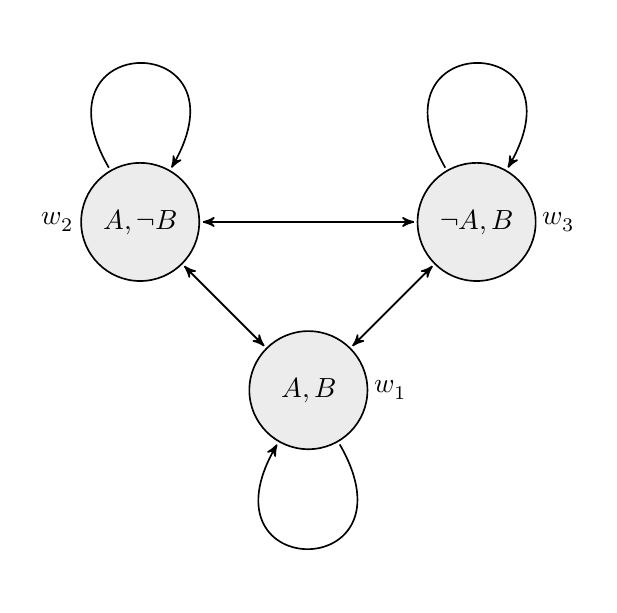
\begin{tikzpicture}[scale=0.6,modal,world/.append style={minimum size=1.5cm}]
      \node[world] (w1) [label=right:$w_1$]{$A,B$}; 
      \node[world] (w2) [label=left:$w_2$, above left=of w1]{$A, \neg B$}; 
      \node[world] (w3) [label=right:$w_3$, above right=of w1] {$\neg A, B$};
      \draw[->] (w1) to (w2);
      \draw[->] (w1) to (w3);
      \draw[->] (w2) to (w1);
      \draw[->] (w3) to (w1);
      \draw[->] (w3) to (w2);
      \draw[->] (w2) to (w3);
      \path[->] (w2) edge[reflexive above] (w2);
      \path[->] (w3) edge[reflexive above] (w3);
      \path[->] (w1) edge[reflexive below] (w1);
    \end{tikzpicture}
    \end{column}
    \begin{column}{0.3\textwidth}
At all points, either $A$ or $B$ is true, so $\Box(A \vee B)$ is true. \pause 

\bigskip

But $\Box A$ and $\Box B$ are false everywhere. \pause So the conditional is false everywhere.
\end{column}
\end{columns}
\end{frame}

\begin{frame}{\(\Box(A \vee B) \rightarrow (\Box A \vee \Box B)\)}
\protect\hypertarget{boxa-vee-b-rightarrow-box-a-vee-box-b-1}{}
\begin{columns}
    \begin{column}{0.65\textwidth}
        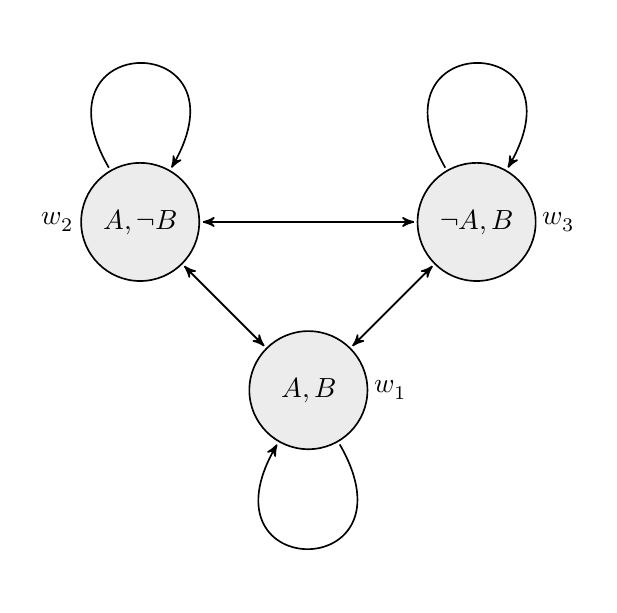
\begin{tikzpicture}[scale=0.6,modal,world/.append style={minimum size=1.5cm}]
      \node[world] (w1) [label=right:$w_1$]{$A,B$}; 
      \node[world] (w2) [label=left:$w_2$, above left=of w1]{$A, \neg B$}; 
      \node[world] (w3) [label=right:$w_3$, above right=of w1] {$\neg A, B$};
      \draw[->] (w1) to (w2);
      \draw[->] (w1) to (w3);
      \draw[->] (w2) to (w1);
      \draw[->] (w3) to (w1);
      \draw[->] (w3) to (w2);
      \draw[->] (w2) to (w3);
      \path[->] (w2) edge[reflexive above] (w2);
      \path[->] (w3) edge[reflexive above] (w3);
      \path[->] (w1) edge[reflexive below] (w1);
    \end{tikzpicture}
    \end{column}
    \begin{column}{0.3\textwidth}
Note that this is overkill. We just need to show that the formula can be false somewhere in order to show that it is not a theorem.
\end{column}
\end{columns}
\end{frame}

\begin{frame}{\((\Diamond A \wedge \Diamond B) \rightarrow \Diamond (A \wedge B)\)}
\protect\hypertarget{diamond-a-wedge-diamond-b-rightarrow-diamond-a-wedge-b}{}
\begin{columns}
    \begin{column}{0.65\textwidth}
        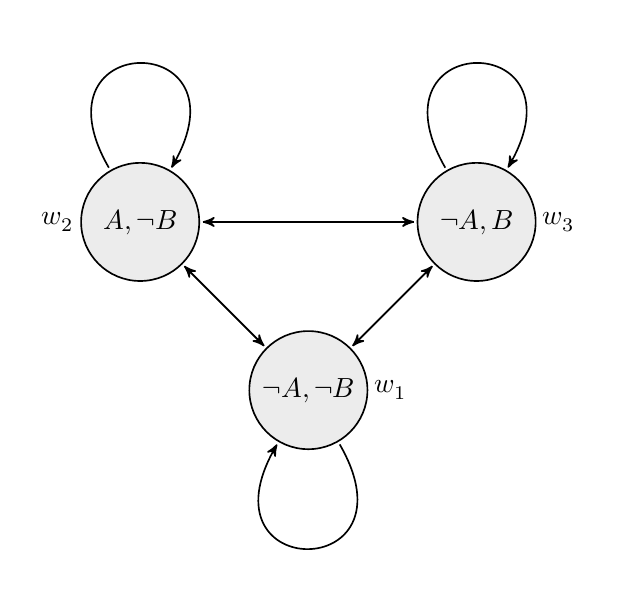
\begin{tikzpicture}[scale=0.5,modal,world/.append style={minimum size=1.5cm}]
      \node[world] (w1) [label=right:$w_1$]{$\neg A, \neg B$}; 
      \node[world] (w2) [label=left:$w_2$, above left=of w1]{$A, \neg B$}; 
      \node[world] (w3) [label=right:$w_3$, above right=of w1] {$\neg A, B$};
      \draw[->] (w1) to (w2);
      \draw[->] (w1) to (w3);
      \draw[->] (w2) to (w1);
      \draw[->] (w3) to (w1);
      \draw[->] (w3) to (w2);
      \draw[->] (w2) to (w3);
      \path[->] (w2) edge[reflexive above] (w2);
      \path[->] (w3) edge[reflexive above] (w3);
      \path[->] (w1) edge[reflexive below] (w1);
    \end{tikzpicture}
    \end{column}
    \begin{column}{0.33\textwidth}

At $w_1$, we have $\Diamond A \wedge \Diamond B$ true. 

\pause \bigskip

But nowhere is $A \wedge B$ true, so $\Diamond(A \wedge B)$ is false at $w_1$. So the conditional is false. 

\pause \bigskip

Again, this is overkill.
\end{column}
\end{columns}
\end{frame}

\begin{frame}{\(A \rightarrow \Box A\)}
\protect\hypertarget{a-rightarrow-box-a}{}
\begin{columns}
    \begin{column}{0.45\textwidth}
        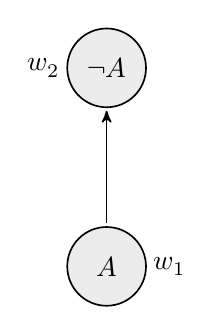
\begin{tikzpicture}[scale=0.6,modal,world/.append style={minimum size=1cm}]
      \node[world] (w1) [label=right:$w_1$]{$A$}; 
      \node[world] (w2) [label=left:$w_2$, above =of w1]{$\neg A$}; 
      \draw[->] (w1) to (w2);
    \end{tikzpicture}
    \end{column}
    \begin{column}{0.5\textwidth}
    \begin{itemize}
    \item At $w_1$ $A$ is true.
    \item But $\Box A$ is false, since $w_1$ can access $w_2$, and $A$ is false there.
    \item So $A \rightarrow \Box A$ is false.
    \end{itemize}
  \end{column}
\end{columns}
\end{frame}

\begin{frame}{\(\Box A \rightarrow A\)}
\protect\hypertarget{box-a-rightarrow-a}{}
\begin{columns}
    \begin{column}{0.45\textwidth}
        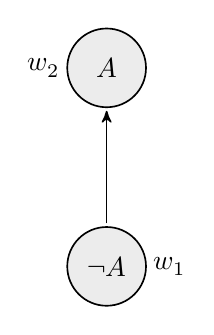
\begin{tikzpicture}[scale=0.6,modal,world/.append style={minimum size=1cm}]
      \node[world] (w1) [label=right:$w_1$]{$\neg A$}; 
      \node[world] (w2) [label=left:$w_2$, above =of w1]{$A$}; 
      \draw[->] (w1) to (w2);
    \end{tikzpicture}
    \end{column}
    \begin{column}{0.5\textwidth}
    \begin{itemize}
    \item At $w_1$ $\Box A$ is true. The only accessible world is $w_2$, and $A$ is true there.
    \item But $A$ is false there.
    \item So $\Box A \rightarrow A$ is false.
    \end{itemize}
  \end{column}
\end{columns}
\end{frame}

\begin{frame}{\(\Box \Diamond A \rightarrow B\)}
\protect\hypertarget{box-diamond-a-rightarrow-b}{}
\begin{columns}
    \begin{column}{0.45\textwidth}
        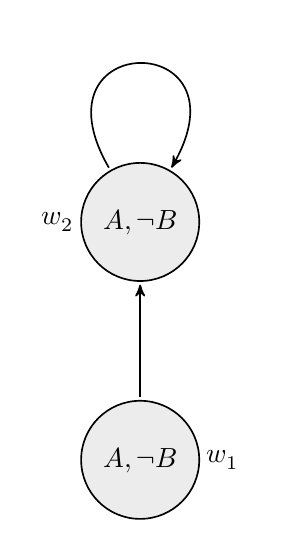
\begin{tikzpicture}[scale=0.6,modal,world/.append style={minimum size=1.5cm}]
      \node[world] (w1) [label=right:$w_1$]{$A, \neg B$}; 
      \node[world] (w2) [label=left:$w_2$, above =of w1]{$A, \neg B$}; 
      \draw[->] (w1) to (w2);
     \path[->] (w2) edge[reflexive above] (w2);
    \end{tikzpicture}
    \end{column}
    \begin{column}{0.5\textwidth}
    \begin{itemize}
    \item At $w_1$ $\Box \Diamond A$ is true. The only accessible world is $w_2$, and $\Diamond A$ is true there. (Why?)
    \item But $B$ is false at $w_1$.
    \item So $\Box \Diamond A \rightarrow B$ is false.
    \end{itemize}
  \end{column}
\end{columns}
\end{frame}

\begin{frame}{\(\Box \Diamond A \rightarrow A\)}
\protect\hypertarget{box-diamond-a-rightarrow-a}{}
\begin{columns}
    \begin{column}{0.45\textwidth}
        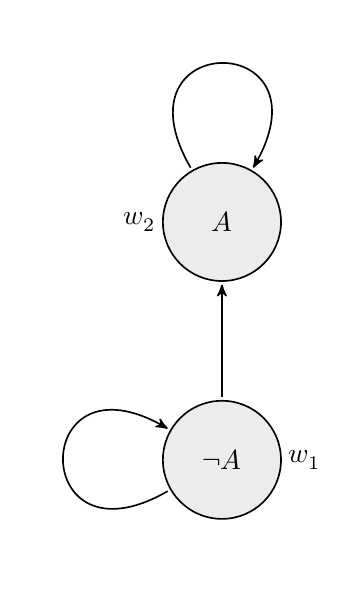
\begin{tikzpicture}[scale=0.6,modal,world/.append style={minimum size=1.5cm}]
      \node[world] (w1) [label=right:$w_1$]{$\neg A$}; 
      \node[world] (w2) [label=left:$w_2$, above =of w1]{$A$}; 
      \draw[->] (w1) to (w2);
     \path[->] (w2) edge[reflexive above] (w2);
     \path[->] (w1) edge[reflexive left] (w1);
    \end{tikzpicture}
    \end{column}
    \begin{column}{0.5\textwidth}
    \begin{itemize}
    \item At $w_1$ $\Box \Diamond A$ is true. At every world, $w_2$ is accessible, and $A$ is true there.
    \item But $A$ is false at $w_1$.
    \item So $\Box \Diamond A \rightarrow A$ is false at $w_1$.
    \end{itemize}
  \end{column}
\end{columns}
\end{frame}

\begin{frame}{\(\Box \Box A \rightarrow \Box A\)}
\protect\hypertarget{box-box-a-rightarrow-box-a}{}
\begin{columns}
    \begin{column}{0.45\textwidth}
        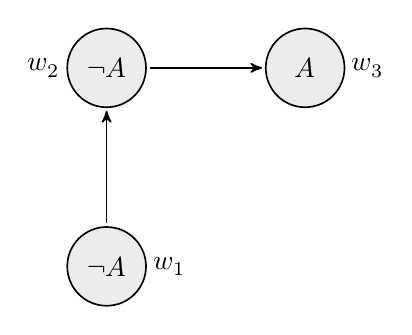
\begin{tikzpicture}[scale=0.5,modal,world/.append style={minimum size=1cm}]
      \node[world] (w1) [label=right:$w_1$]{$\neg A$}; 
      \node[world] (w2) [label=left:$w_2$, above =of w1]{$\neg A$}; 
      \node[world] (w3) [label=right:$w_3$, right =of w2]{$A$}; 
      \draw[->] (w1) to (w2);
      \draw[->] (w2) to (w3);
%     \path[->] (w2) edge[reflexive above] (w2);
%     \path[->] (w1) edge[reflexive left] (w1);
    \end{tikzpicture}
    \end{column}
    \begin{column}{0.5\textwidth}
    \begin{itemize}
    \item The only world $w_2$ can access is $w_3$, and $A$ is true there, so $\Box A$ is true at $w_2$.
    \item The only world $w_1$ can access is $w_2$, and $\Box A$ is true there, so $\Box \Box A$ is true at $w_1$.
    \item But $\Box A$ is false at $w_1$.
    \item So $\Box \Box A \rightarrow \Box A$ is false at $w_1$.
    \end{itemize}
  \end{column}
\end{columns}
\end{frame}

\begin{frame}{\(\Box A \rightarrow \Box \Box A\)}
\protect\hypertarget{box-a-rightarrow-box-box-a}{}
\begin{columns}
    \begin{column}{0.45\textwidth}
        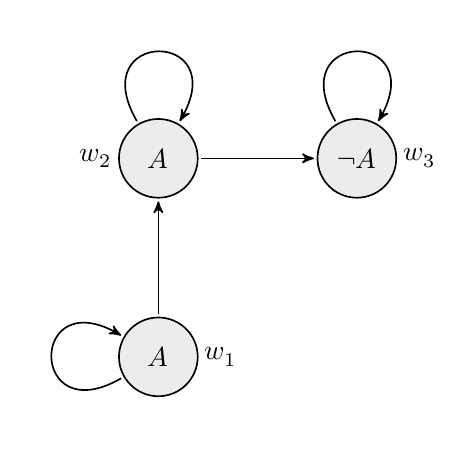
\begin{tikzpicture}[scale=0.5,modal,world/.append style={minimum size=1cm}]
      \node[world] (w1) [label=right:$w_1$]{$A$}; 
      \node[world] (w2) [label=left:$w_2$, above =of w1]{$A$}; 
      \node[world] (w3) [label=right:$w_3$, right =of w2]{$\neg A$}; 
      \draw[->] (w1) to (w2);
      \draw[->] (w2) to (w3);
     \path[->] (w2) edge[reflexive above] (w2);
     \path[->] (w3) edge[reflexive above] (w3);
     \path[->] (w1) edge[reflexive left] (w1);
    \end{tikzpicture}
    \end{column}
    \begin{column}{0.5\textwidth}
    \begin{itemize}
    \item Since $A$ is false at $w_3$, and $w_2$ can access $w_3$, $\Box A$ is false at $w_2$.
    \item Since $\Box A$ is false at $w_2$, and $w_1$ can access $w_2$, $\Box \Box A$ is false at $w_1$.
    \item But $\Box A$ is true at $w_1$.
    \item So $\Box A \rightarrow \Box \Box A$ is false at $w_1$.
    \end{itemize}
       \end{column}
\end{columns}
\end{frame}

\begin{frame}{\(\Box A \rightarrow \Diamond A\)}
\protect\hypertarget{box-a-rightarrow-diamond-a}{}
\begin{columns}
    \begin{column}{0.45\textwidth}
        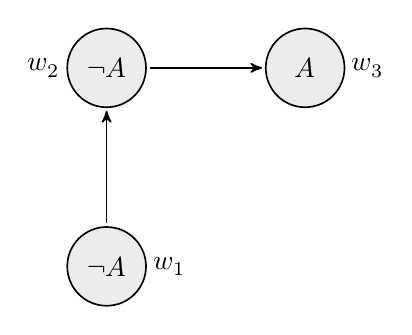
\begin{tikzpicture}[scale=0.5,modal,world/.append style={minimum size=1cm}]
      \node[world] (w1) [label=right:$w_1$]{$\neg A$}; 
      \node[world] (w2) [label=left:$w_2$, above =of w1]{$\neg A$}; 
      \node[world] (w3) [label=right:$w_3$, right =of w2]{$A$}; 
      \draw[->] (w1) to (w2);
      \draw[->] (w2) to (w3);
%     \path[->] (w2) edge[reflexive above] (w2);
%     \path[->] (w1) edge[reflexive left] (w1);
    \end{tikzpicture}
    \end{column}
    \begin{column}{0.5\textwidth}
    \begin{itemize}
    \item Focus on $w_3$.
    \item There is no accessible world where $A$ is false, so $\Box A$ is true there.
    \item But there is no accessible world where $A$ is true, so $\Diamond A$ is false there.
    \item So $\Box A \rightarrow \Diamond A$ is false there.
    \end{itemize}
\end{column}
\end{columns}
\end{frame}

\begin{frame}{\(\Box A \rightarrow \Diamond A\)}
\protect\hypertarget{box-a-rightarrow-diamond-a-1}{}
\begin{columns}
    \begin{column}{0.45\textwidth}
        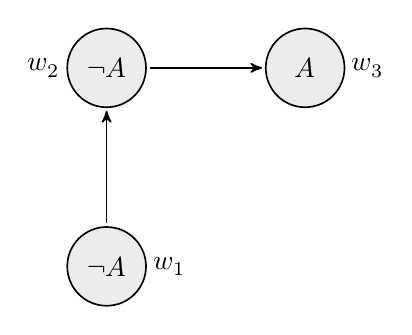
\begin{tikzpicture}[scale=0.5,modal,world/.append style={minimum size=1cm}]
      \node[world] (w1) [label=right:$w_1$]{$\neg A$}; 
      \node[world] (w2) [label=left:$w_2$, above =of w1]{$\neg A$}; 
      \node[world] (w3) [label=right:$w_3$, right =of w2]{$A$}; 
      \draw[->] (w1) to (w2);
      \draw[->] (w2) to (w3);
%     \path[->] (w2) edge[reflexive above] (w2);
%     \path[->] (w1) edge[reflexive left] (w1);
    \end{tikzpicture}
    \end{column}
    \begin{column}{0.5\textwidth}
    Whenever there are no accessible worlds, the following two weird things happen.
    \begin{enumerate}
    \item All $\Box$-sentences (i.e., sentences that start with a $\Box$ that takes scope over the whole sentence) are true.
    \item All $\Diamond$-sentences (i.e., sentences that start with a $\Diamond$ that takes scope over the whole sentence) are false.
    \end{enumerate}
   \end{column}
\end{columns}
\end{frame}



\end{document}
